\section{File System Implementation}

\paragraph{Disk Structure}
\begin{items}
  \item \textbf{partitions}: disk can be subdivided into partitions
  \item \textbf{raw usage}: disks/partitions can be used raw (unformatted) or formatted with file system
  \item \textbf{volume}: entry containing FS \\*
    $ - $ tracks that file system's info is in device directory or volume table of contents
  \item \textbf{FS diversity}: there are general purpose and special purpose FS
\end{items}

\paragraph{File Systems --- logical vs. physical}
\begin{items}
  \item \textbf{logical}: can consist of different physical file systems
  \item \textbf{placement}: file system can be mounted at any place within another file system
  \item \textbf{mounted local root}: bit in i-node of local root in mounted file system identifies this directory as mount point
\end{items}

\paragraph{File Systems --- layers}
\begin{items}
  \item \textbf{layer 5}: applications
  \item \textbf{layer 4}: logical file system
  \item \textbf{layer 3}: file-organization module
  \item \textbf{layer 2}: basic file system
  \item \textbf{layer 1}: I/O control
  \item \textbf{layer 0}: devices
\end{items}

\paragraph{File Systems --- virtual}
\begin{items}
  \item \textbf{principle}: provide object-oriented way of implementing file systems \\*
    $ - $ same API used for different file system types
\end{items}
\begin{figure}[H]\centering\label{VirtualFileSystem}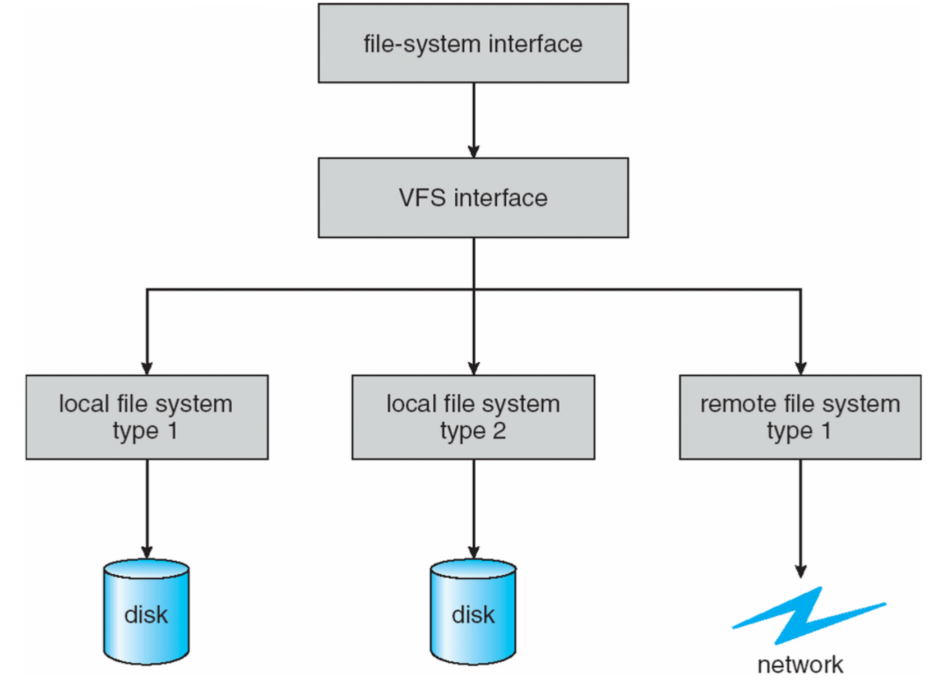
\includegraphics[width=0.33\textwidth]{VirtualFileSystem}\end{figure}

\paragraph{Files --- implementation}
\begin{items}
  \item \textbf{meta data} must be tracked: \\*
    $ - $ which logical block belongs to which file? \\*
    $ - $ block order? \\*
    $ - $ which blocks are free for next allocation?
  \item \textbf{block identification}: blocks on disk must be identified by FS (given logical region of file) \\*
    $ \to $ meta data needed in \emph{file allocation table}, \emph{directory} and \emph{inode}
  \item \textbf{block management}: creating/updating files might imply allocating new/modifying old disk blocks
\end{items}

\paragraph{Allocation --- policies}
\begin{items}
  \item \textbf{preallocation}: \\*
    $ - $ \emph{problem}: need to know maximum file size at creation time \\*
    $ - $ often difficult to reliably estimate maximum file size \\*
    $ - $ users tend to overestimate file size to avoid running out of space
  \item \textbf{dynamic allocation}: allocate in pieces as needed
\end{items}

\paragraph{Allocation --- fragment size}
\begin{items}
  \item \textbf{extremes}: \\*
    $ - $ fragment size = length of file \\*
    $ - $ fragment size = smallest disk block size (= sector size)
  \item \textbf{trade-offs}: \\*
    $ - $ \emph{contiguity}: speedup for sequential accesses \\*
    $ - $ \emph{small fragments}: larger tables needed to manage free storage and file access \\*
    $ - $ \emph{large fragments}: improve data transfer \\*
    $ - $ \emph{fixed-size fragments}: simplifies space reallocation \\*
    $ - $ \emph{variable-size fragments}: minimizes internal fragmentation, can lead to external fragmentation
\end{items}

\paragraph{Allocation --- file space}
\begin{items}
  \item \textbf{contiguous}
  \item \textbf{chained}
  \item \textbf{indexed}: \\*
    $ - $ fixed block fragments \\*
    $ - $ variable block fragments
\end{items}
\begin{figure}[H]\centering\label{AllocationOverview}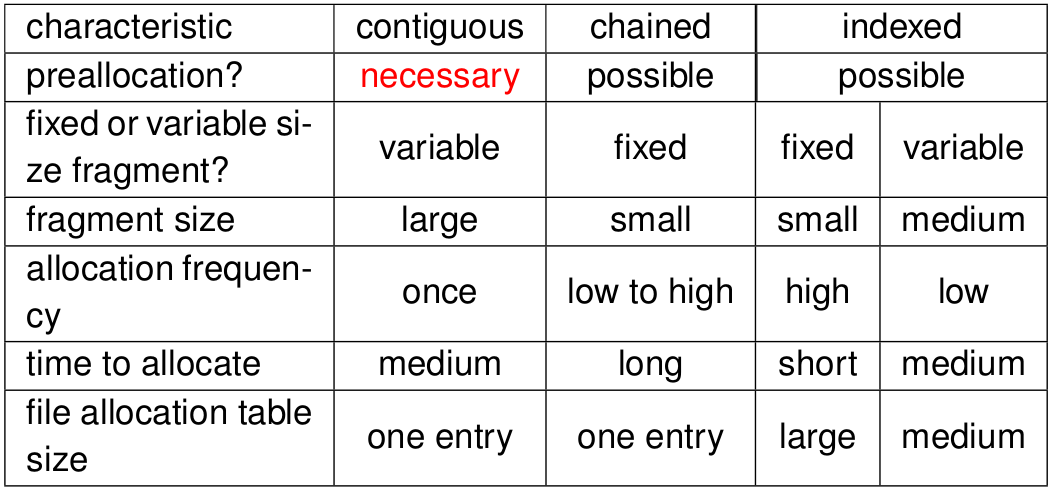
\includegraphics[width=0.33\textwidth]{AllocationOverview}\end{figure}

\paragraph{Allocation --- contiguous}
\begin{items}
  \item \textbf{principle}: array of $ n $ contiguous logical blocks reserved per file (to be created)
  \item \textbf{periodic compaction}: overcome external fragmentation
\end{items}
\begin{figure}[H]\centering\label{AllocationContiguous}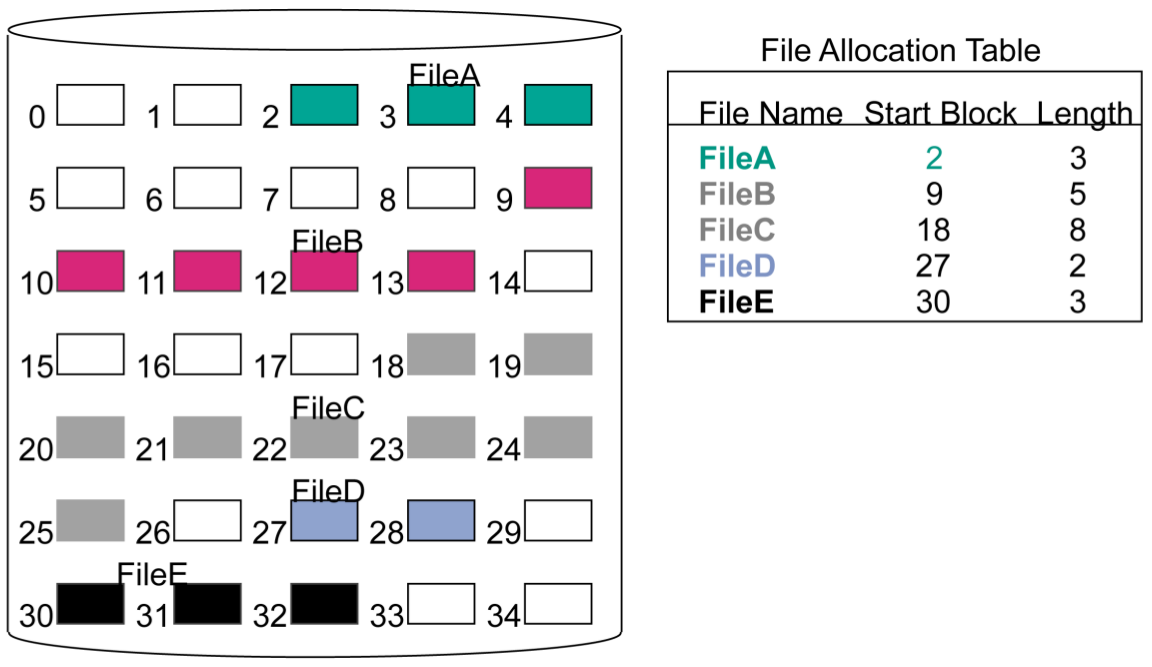
\includegraphics[width=0.33\textwidth]{AllocationContiguous}\end{figure}

\paragraph{Allocation --- chained}
\begin{items}
  \item \textbf{principle}: linked list of logical blocks per file \\*
    $ - $ FAT or directory contains address of first file block \\*
    $ \to $ \emph{no external fragmentation}: any free block can be added to chain
\end{items}
\begin{figure}[H]\centering\label{AllocationChained}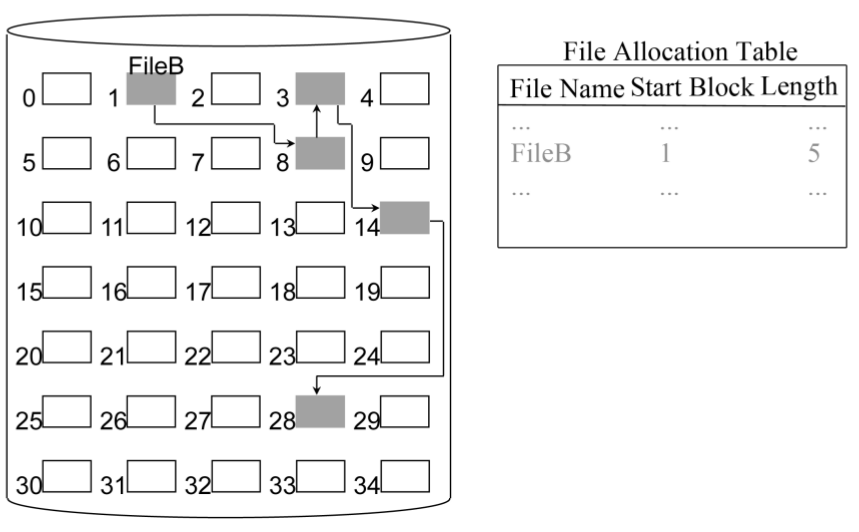
\includegraphics[width=0.33\textwidth]{AllocationChained}\end{figure}

\paragraph{Allocation --- indexed}
\begin{items}
  \item \textbf{principle}: FAT contains one-level index table per file \\*
    $ - $ \emph{generalization}: $ n $-level index table \\*
    $ - $ index has one entry for allocated file block \\*
    $ - $ FAT contains block number for index
\end{items}
\begin{figure}[H]\centering\label{AllocationIndexed}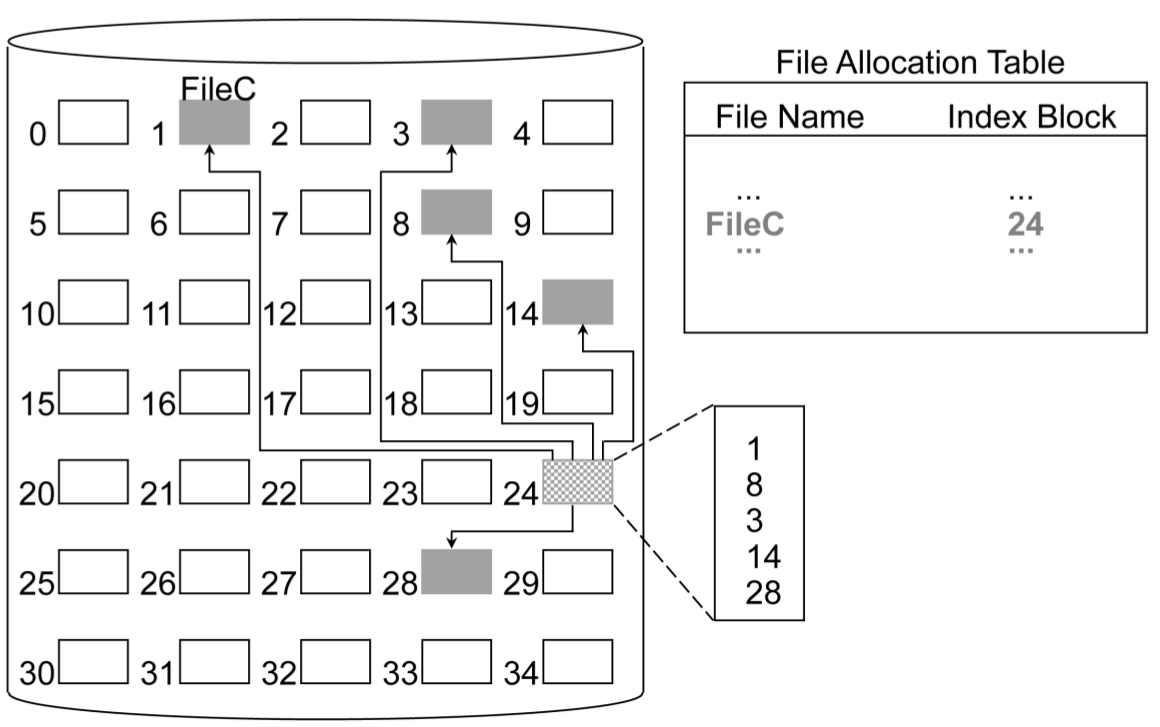
\includegraphics[width=0.33\textwidth]{AllocationIndexed}\end{figure}

\paragraph{Directories --- implementation}
\begin{items}
  \item \textbf{simple directory} (MS-DOS): \\*
    $ - $ fixed-size entries \\*
    $ - $ disk addresses + attributes in directory entry
  \item \textbf{i-node reference directory} (UNIX): \\*
    $ - $ entry refers to i-node containing attributes
\end{items}

\paragraph{Disk Blocks --- buffering}
\begin{items}
  \item \textbf{buffering}: disk blocks buffered in main memory
  \item \textbf{access}: buffer access done via hash table \\*
    $ - $ blocks with same hash value are chained together
  \item \textbf{replacement}: LRU
  \item \textbf{management}: free buffer is managed via doubly-linked list
\end{items}

\paragraph{File Systems --- journaling}
\begin{items}
  \item \textbf{principle}: record each update to file system as \emph{transaction} \\*
    $ - $ written to log
  \item \textbf{committed} transaction = written to log \\*
    $ \to $ \emph{problem}: file system may not yet be updated
  \item \textbf{writing} transactions from log to FS is asynchronous
  \item \textbf{modifying} FS $ \to $ transaction removed from log
  \item \textbf{crash} of file system $ \to $ remaining transactions in log must still be performed
\end{items}

\paragraph{File Systems --- log-structured}
\begin{items}
  \item \textbf{principle}: use disk as circular buffer \\*
    $ - $ write all updated (including i-nodes, meta data and data) to end of log
  \item \textbf{buffering}: all writes initially buffered in memory
  \item \textbf{writing}: periodically write within 1 segment (1 MB)
  \item \textbf{opening}: locate i-node, find blocks
  \item \textbf{clearing}: clear all data from other end, no longer used
\end{items}